
\chapter{Hardware}

\section{Design}
\subsection{Forstærkning}
\subsection{Lavpas}
I projektet skal der laves et 2. ordens lavpasfilter. Dette filter skal være et Buttenworth-filter, med en knækfrekvens på 50 Hz. 

\section{Implementering}
\subsection{Forstærkning}
\subsection{Lavpas}


\section{Modultest}
\subsection{Forstærkning}
\subsection{Lavpas}
For at teste lavpasfilteret foretages målinger med en sinus, hvor frekvensen variere for hver måling. Derved aflæses fasen, mellem indgang- og udgangssignal, og amplituden for hver måling.  
\begin{figure}[htb]
	\centering
	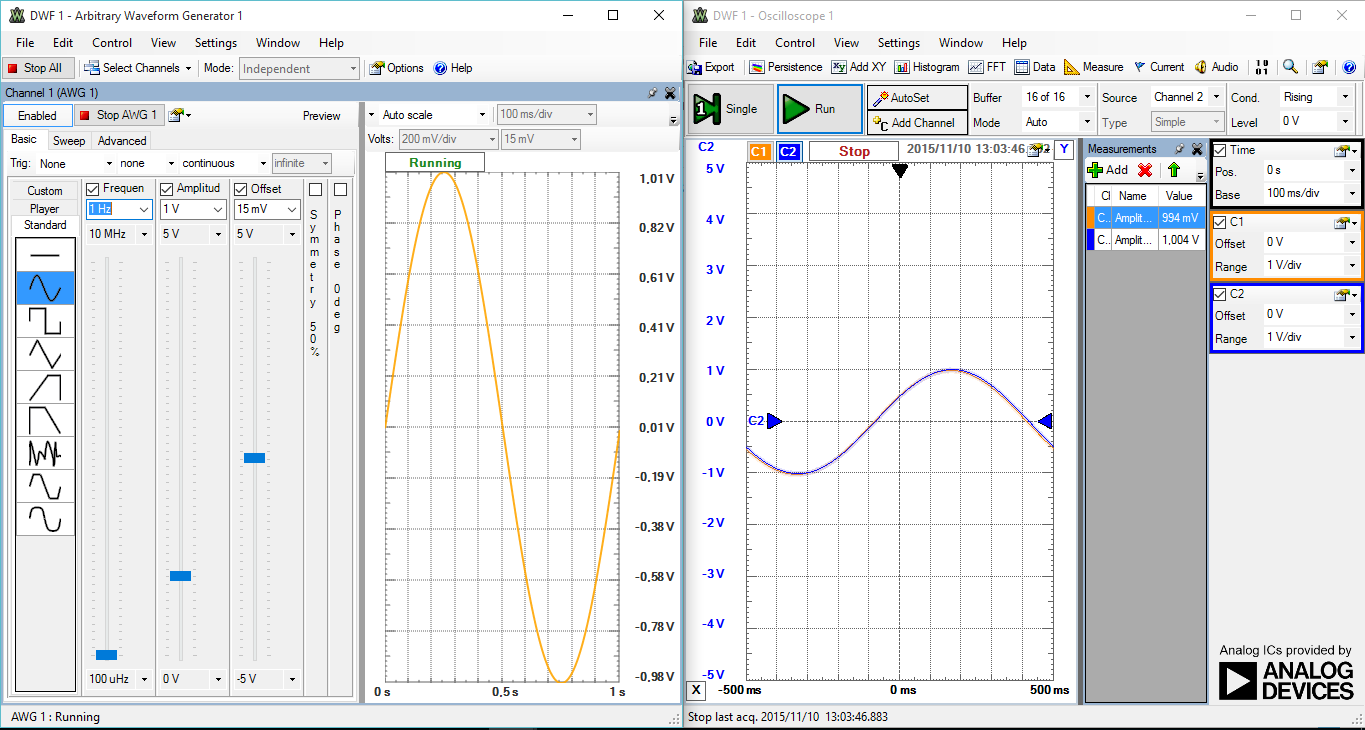
\includegraphics[width=1.0\textwidth]{Figurer/10Hz}
	\caption{Måling for 10 Hz}
	\label{fig:maeling10Hz}
\end{figure}
